% ============================================================================
% 第 6 章 系统功能模块详细实现
% ============================================================================
\chapter{系统功能模块详细实现}

在总体架构与 AI Agent 核心机制确定后，系统功能实现按照学生端、教师端、管理员端与公共模块四条线展开。前端使用 Vue 3、TypeScript、Element Plus 与 ECharts，后端使用 Spring Boot、Spring Security、MyBatis-Plus、Redis、MinIO 与 DashScope 兼容接口。各端页面并非独立孤立实现，而是围绕病例、训练记录、评分和用户权限形成统一的数据流。

% ----------------------------------------------------------------------------
\section{学生端核心模块}

\subsection{AI 问诊训练界面}

学生端的核心页面是 AI 问诊训练界面，对应前端 \texttt{student/Consultation.vue} 与 \texttt{student/Training.vue} 等页面。如图~\ref{fig:student_consultation_ui} 所示，该界面采用左右分区布局：左侧为病例摘要、训练状态和可用临床资料入口；右侧为对话区、输入框和操作按钮。学生进入训练后，前端先调用 \texttt{/api/training/start} 创建训练记录，再以记录 ID 调用 \texttt{/api/chat/send} 或流式接口发送问诊内容。

\begin{figure}[H]
    \centering
    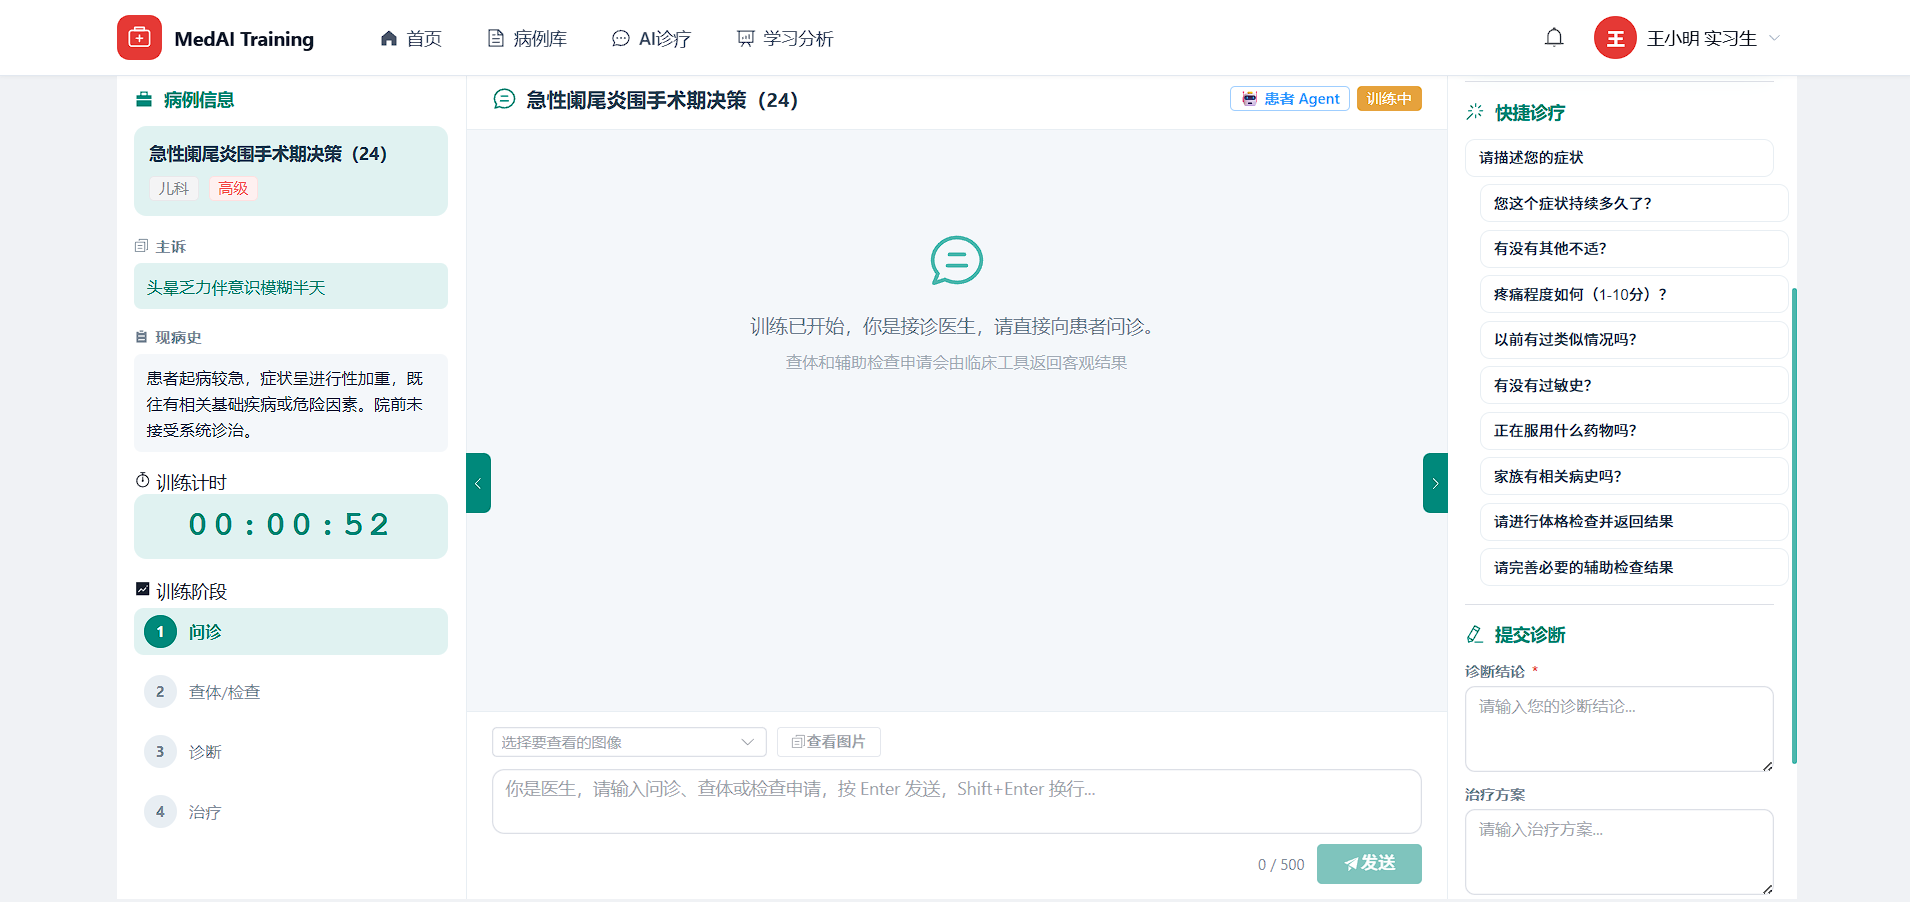
\includegraphics[width=0.9\textwidth]{figures/虚拟问诊系统学生端会诊界面图.png}
    \caption{学生端 AI 问诊训练界面}
    \label{fig:student_consultation_ui}
\end{figure}

该模块的实现重点有三点。第一，聊天记录按发送方区分气泡样式，学生消息、AI 回复、临床工具结果在视觉上区分，便于学生复盘。第二，前端对流式响应进行增量渲染，避免大模型响应期间页面长时间空白。第三，训练过程中的检查请求不会直接交给大模型生成，而是由后端临床工具返回病例中录入的客观检查结果，保证教学数据的一致性。

\subsection{病例选择与训练启动}

病例选择模块对应病例列表与详情页面。学生可根据科室、难度、关键词等条件浏览病例，查看标题、病例简介、学习目标、预计学时和训练次数等信息。病例详情页不展示参考诊断和治疗方案，只展示可用于选择训练的非泄题信息，防止学生在开始训练前获得标准答案。

训练启动时，前端向 \texttt{/api/training/start} 提交病例 ID 和训练模式，后端在 \texttt{TrainingServiceImpl.startTraining()} 中校验病例是否存在、是否发布，并创建一条 \texttt{training\_record}。训练记录状态初始为进行中，记录开始时间、用户 ID、病例 ID 和训练模式。创建成功后前端跳转到问诊界面，并将 \texttt{recordId} 作为后续对话、提交诊断和查看报告的主键。

\subsection{学习分析与雷达图}

学习分析模块负责把多次训练结果转化为可视化反馈。后端 \texttt{AnalysisController} 提供学生维度的学习分析接口，前端通过 ECharts 雷达图展示问诊、诊断、治疗和沟通四个能力维度，通过折线图展示成绩变化趋势，通过列表展示薄弱知识点与推荐训练病例。学习分析界面如图~\ref{fig:student_analysis} 所示。

\begin{figure}[H]
    \centering
    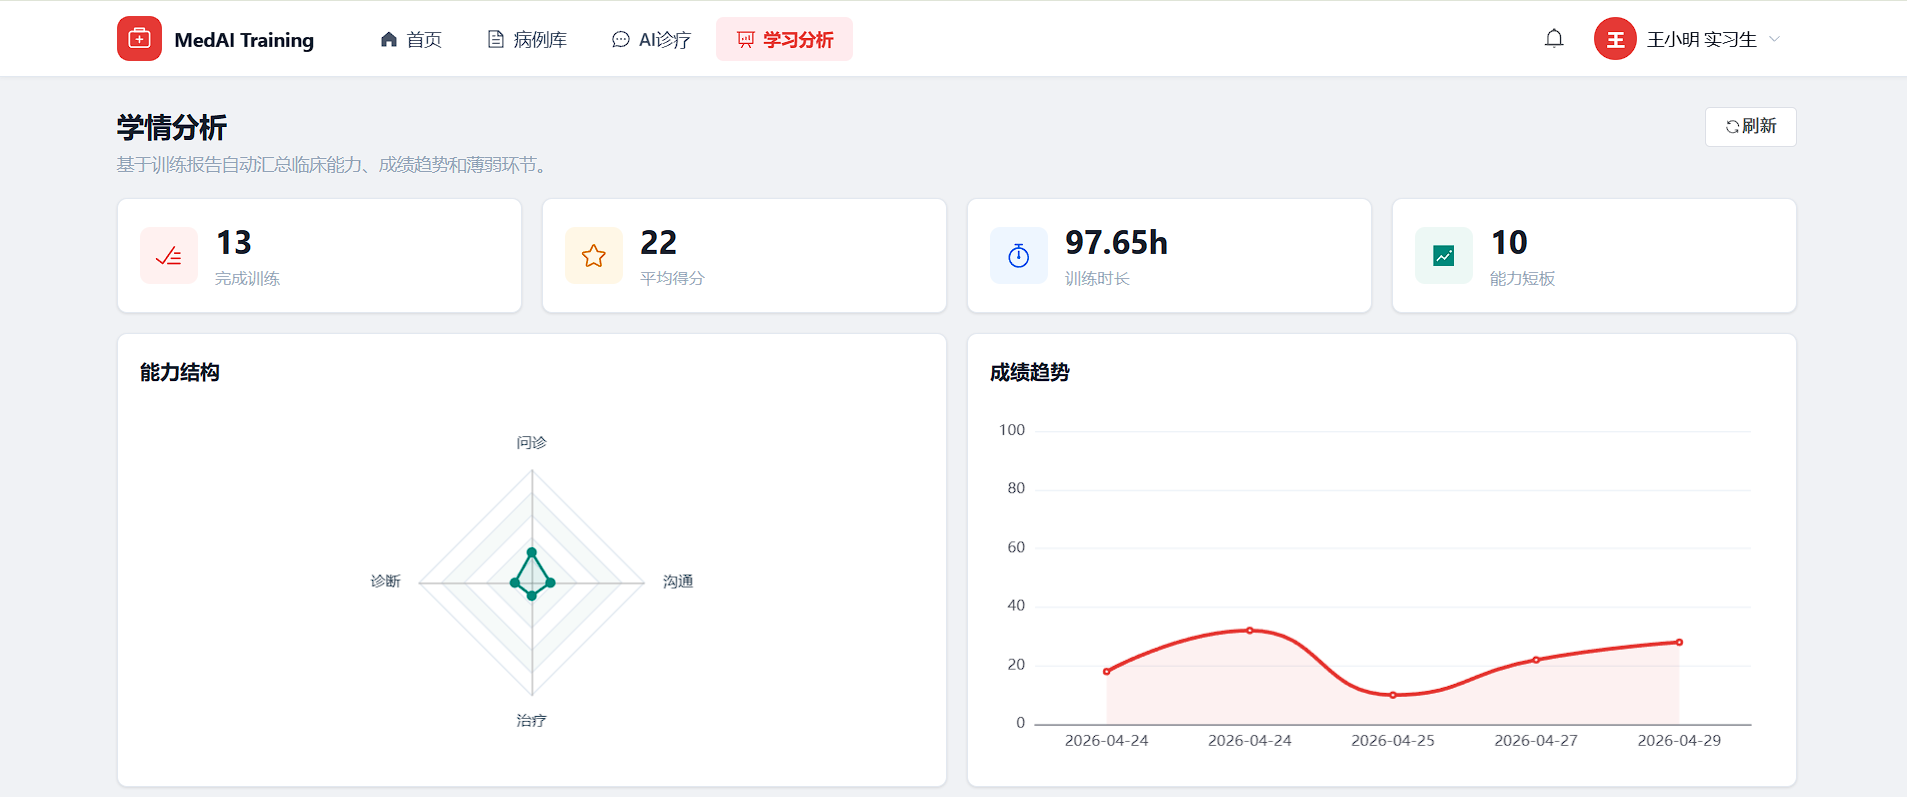
\includegraphics[width=0.9\textwidth]{figures/虚拟问诊系统学生端学情分析界面图.png}
    \caption{学生端学习分析界面}
    \label{fig:student_analysis}
\end{figure}

学习分析不只展示分数，还承担“下一步怎么练”的指导功能。系统根据训练评分中的 \texttt{weakPoints}、\texttt{errorPatterns} 和病例科室信息，帮助学生发现反复出错的环节。例如，如果多次训练中诊断得分偏低，系统会提示学生补强鉴别诊断和诊断依据表达；如果问诊得分偏低，则建议围绕主诉、现病史、既往史、个人史和家族史构建完整问诊模板。

% ----------------------------------------------------------------------------
\section{教师端核心模块}

图~\ref{fig:teacher_home} 展示了教师端首页界面，教师可以通过该界面快速访问病例管理、班级管理、成绩批改和教学分析等功能。

\begin{figure}[H]
    \centering
    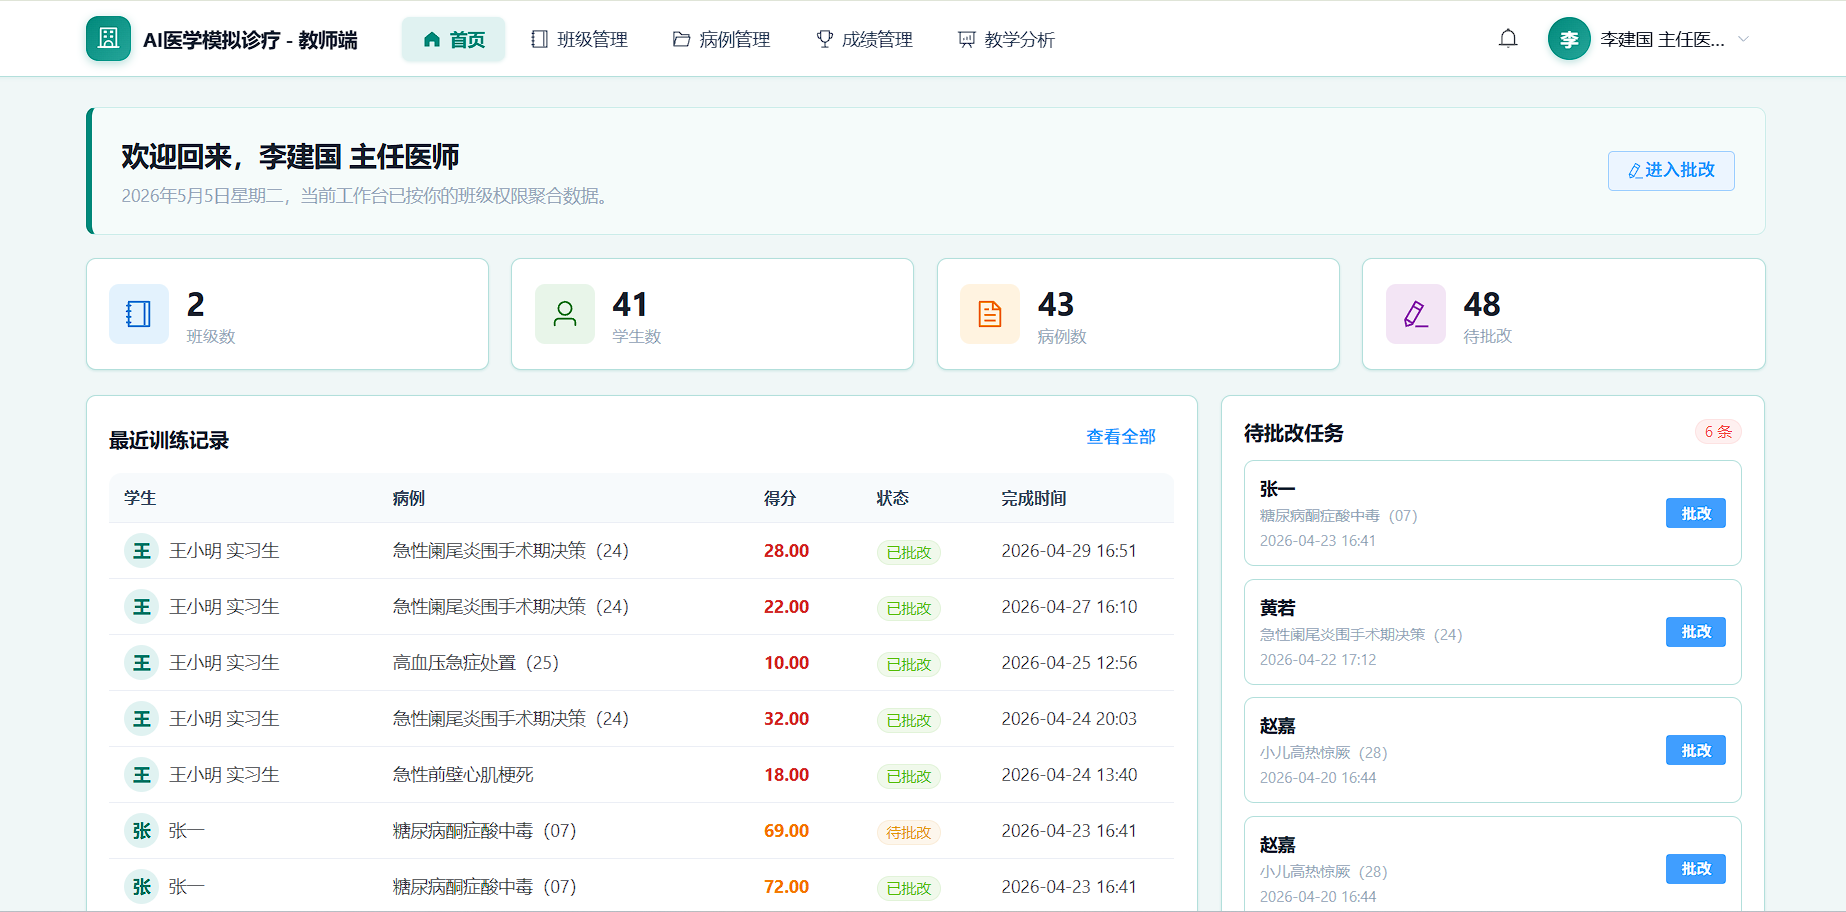
\includegraphics[width=0.9\textwidth]{figures/虚拟问诊系统教师端首页界面图.png}
    \caption{教师端首页界面}
    \label{fig:teacher_home}
\end{figure}

\subsection{病例管理与多媒体上传}

教师端病例管理模块对应 \texttt{teacher/CaseManagement.vue} 与 \texttt{CaseController}。教师可以创建、编辑、发布和归档病例，填写主诉、现病史、既往史、体格检查、辅助检查、参考诊断、参考治疗方案、学习目标和评分标准等信息。病例状态分为草稿、已发布和已归档，只有已发布病例对学生可见。

医学影像和附件通过文件上传接口进入 MinIO 对象存储，病例表中保存附件 URL、类型和文件名等元信息。上传模块需要关注两类约束：一是文件大小和文件类型限制，避免非预期文件进入对象存储；二是影像类型标注，例如胸片、CT、心电图、检验报告等，用于后端临床工具自动匹配学生请求。

\subsection{批改工作台}

批改工作台对应 \texttt{teacher/ReviewWorkbench.vue} 与 \texttt{GradeController}。教师可以查看学生训练记录、对话全过程、AI 自动评分、薄弱点、错误模式和改进建议，并在此基础上填写教师评分和评语。AI 评分用于提高批改效率，但最终教学评价仍保留教师复核入口。

工作台的实现重点是“过程可追溯”。教师不仅能看到最终分数，还能看到学生每一轮问诊、检查请求、AI 回复和临床工具返回结果。这样，教师可以判断学生是否真正按照临床思维推进问诊，而不是只依据最终提交的诊断和治疗方案打分。

\subsection{教学分析}

教学分析模块对应 \texttt{teacher/TeachingAnalysis.vue}。该模块以班级为统计单位，展示班级平均成绩、各能力维度雷达图、知识点错误分布和训练参与情况。教师可通过筛选班级、时间范围和科室查看不同群体的训练表现。

教学分析的价值在于从个体反馈扩展到群体教学决策。例如，当某班级在治疗方案维度普遍偏低时，教师可以安排专题讲解；当多个学生在同一知识点上出现错误时，系统可以将该知识点列为课堂复盘重点。这使 AI 问诊训练不再只是学生个人练习工具，也能反向服务课程教学改进。

% ----------------------------------------------------------------------------
\section{管理员端核心模块}

图~\ref{fig:admin_overview} 展示了管理员端系统概览界面，管理员可以通过该界面查看系统运行状态和业务数据总览。

\begin{figure}[H]
    \centering
    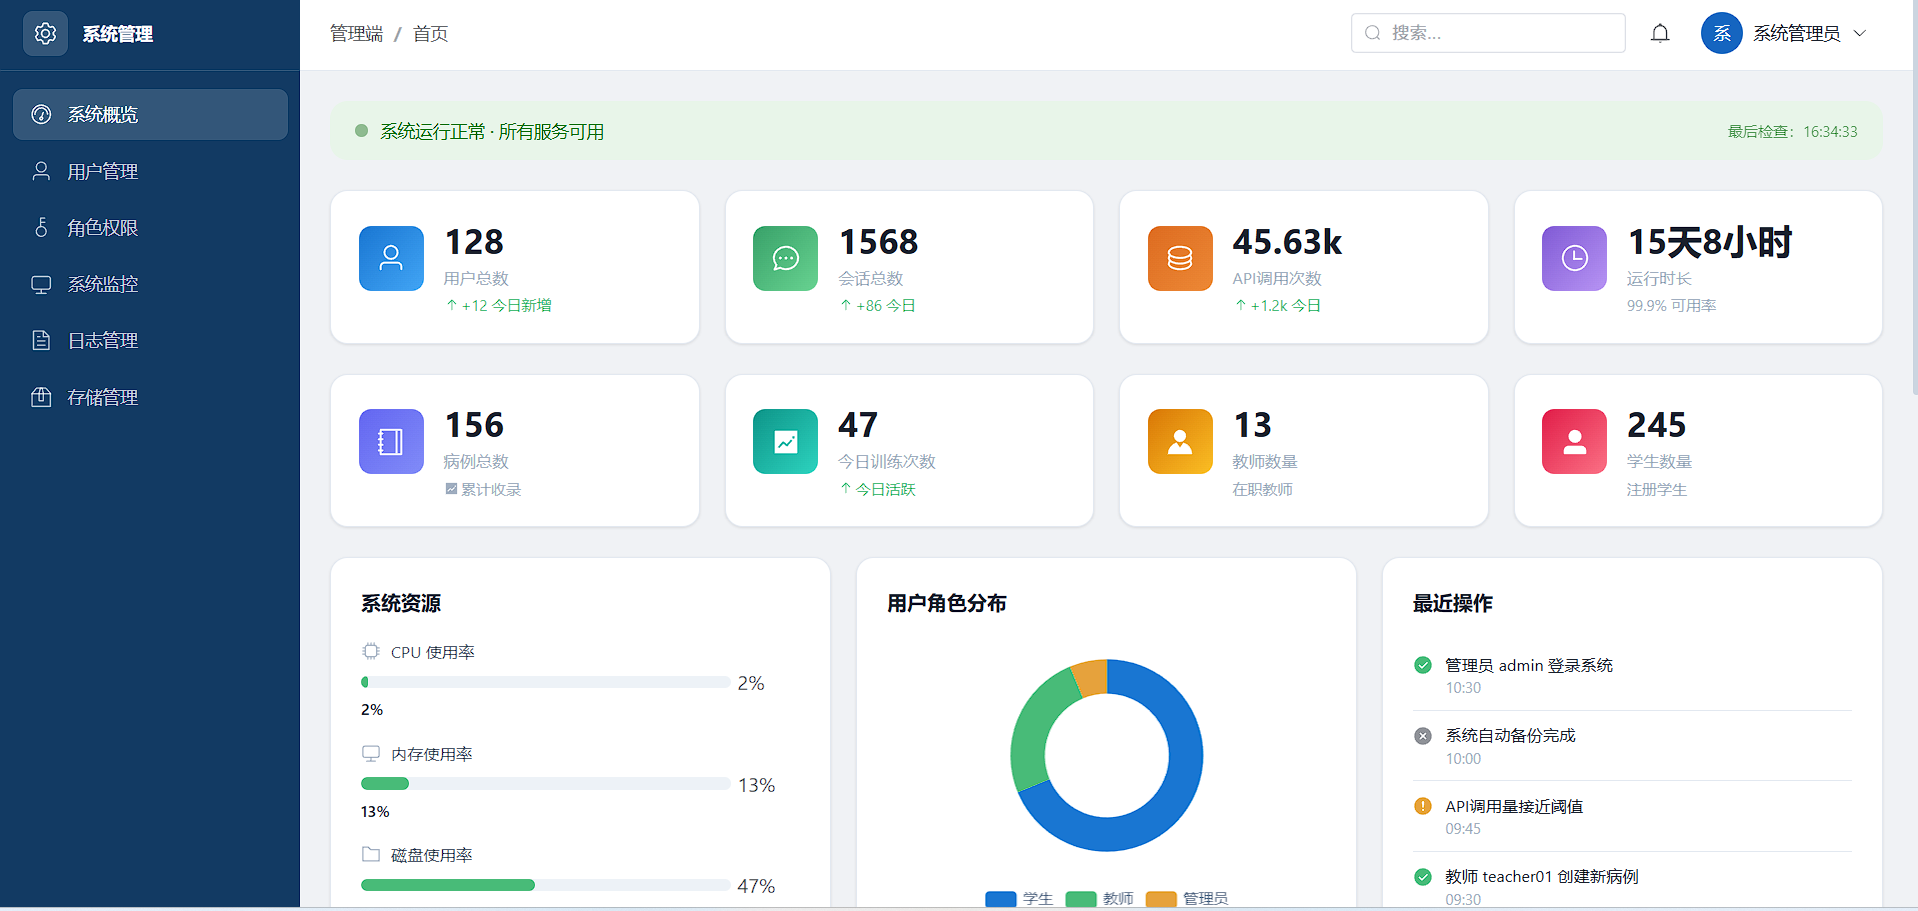
\includegraphics[width=0.9\textwidth]{figures/虚拟问诊系统管理端系统概览界面图.png}
    \caption{管理员端系统概览界面}
    \label{fig:admin_overview}
\end{figure}

\subsection{用户与角色管理}

管理员端用户管理模块对应 \texttt{admin/UserManagement.vue} 与 \texttt{AdminController}。管理员可以查询用户、创建用户、编辑用户信息、禁用或启用账号、重置密码，并按角色、状态、关键词等条件筛选。角色管理模块维护 \texttt{super\_admin}、\texttt{admin}、\texttt{teacher} 和 \texttt{student} 等角色，为后续菜单权限和接口权限扩展提供基础。

用户管理模块与安全模块紧密相关。密码在数据库中不保存明文，而是通过 BCrypt 进行哈希；登录失败次数与锁定状态由 Redis 管理；管理员重置密码会记录操作日志，便于审计。

\subsection{系统监控}

系统监控模块对应 \texttt{admin/SystemMonitor.vue} 与 \texttt{/api/admin/monitor/*} 接口，主要展示服务运行状态、在线用户数、业务数据总量、CPU、内存、磁盘、Redis 与数据库连接状态等信息。系统部署在 Docker Compose 环境下，管理员可通过监控页面快速判断后端、数据库、缓存和对象存储是否正常。

该模块不是完整的专业运维平台，而是为教学系统提供轻量级运行可视化。对于毕业设计答辩和后续课程演示而言，监控页面可以直接说明系统不是单机静态页面，而是由前端、后端、数据库、缓存和对象存储共同构成的可运行应用。

\subsection{日志与存储管理}

日志管理模块记录用户登录、病例编辑、成绩批改、权限变更、文件上传等关键操作。后端通过 \texttt{@OperationLog} 注解和 AOP 切面采集请求路径、请求方法、用户 ID、用户名、IP、耗时、状态和错误信息，并对密码、token、验证码等敏感字段脱敏。日志可用于排查问题，也可作为教学系统合规运行的审计依据。

存储管理模块面向 MinIO 文件资源，提供文件列表、下载、删除和存储统计能力。医学影像与病例附件体积较大，不适合直接存入 MySQL，因此系统采用“对象存储保存文件、数据库保存元信息”的方式，兼顾性能与可维护性。

% ----------------------------------------------------------------------------
\section{公共模块}

\subsection{认证授权}

认证授权模块贯穿学生端、教师端和管理员端。用户登录时，前端提交用户名、密码和验证码，后端先通过验证码服务校验 Redis 中的验证码，再通过认证服务校验用户名和密码，成功后生成 JWT 返回前端。之后前端在授权请求头中携带令牌，后端过滤器解析令牌并写入安全上下文。

% TODO: 此处需要插入登录认证时序图（原 TikZ 箭头和标签重叠，已删除）
% \begin{figure}[htbp]
%     \centering
%     \includegraphics[width=0.85\textwidth]{figures/login_sequence.png}
%     \caption{登录认证时序图}
%     \label{fig:login_sequence}
% \end{figure}

在权限控制上，前端通过路由守卫限制不同角色访问不同页面，后端通过 Spring Security 保护除登录、注册、验证码、健康检查和文件预览外的大多数接口。对于训练记录、成绩和班级数据，后端还在业务层做资源归属校验，避免用户越权访问他人数据。

\subsection{文件上传}

文件上传模块主要服务于病例附件、医学影像和用户头像。前端通过表单上传文件，后端接收后调用 MinIO 客户端保存对象，并返回可访问 URL。病例管理页面会将 URL 与附件类型一起保存到病例信息中，训练过程中临床工具可以根据附件类型匹配学生请求。

为保证安全性，系统限制上传文件大小，并在业务层根据使用场景校验文件类型。对于医学影像类附件，前端展示时不直接暴露对象存储内部路径，而是通过后端预览接口或公共访问地址生成可控链接。

\subsection{数据可视化}

数据可视化模块主要使用 ECharts 实现，包括学生端能力雷达图、成绩趋势折线图、教师端班级平均分柱状图、知识点错误分布图和管理员端系统运行状态图。可视化数据均由后端分析接口返回，前端只负责展示和交互。

相比纯列表展示，可视化模块更适合医学实训的复盘场景。学生可以快速识别自己的短板，教师可以观察班级整体能力结构，管理员可以掌握系统运行状态。该模块与 AI 评分结果、训练记录和班级关系共同构成系统的数据闭环。

% ----------------------------------------------------------------------------
\section{本章小结}

本章从功能实现角度说明了系统的主要模块。学生端围绕病例选择、AI 问诊训练和学习分析形成学习闭环；教师端围绕病例管理、批改工作台和教学分析形成教学闭环；管理员端围绕用户、监控、日志和存储形成运维闭环；公共模块提供认证、文件和可视化基础能力。上述功能共同支撑了第 5 章所述 AI Agent 能力在真实业务界面中的落地。
